\points{3c} \textbf{Denoising Score Matching}

\textbf{Denoising Score Matching (DSM)} enhances Exact Score Matching by addressing the computational challenges associated with directly estimating the trace of 
the Jacobian of the score function. In Exact Score Matching, the trace of the Jacobian matrix can be computationally expensive and 
unstable in high dimensions. DSM avoids this by introducing Gaussian noise to the data and training the model to predict the score of 
the noisy data distribution. This approach indirectly aligns the score function of the model with the true data distribution without 
requiring explicit computation of the Jacobian.

The DSM objective is mathematically defined as:
\begin{align}    
    \mathcal{L}_{\text{denoising}} = \mathbb{E}_{x \sim p_{\text{data}(x)}} \mathbb{E}_{z \sim \mathcal{N}(0, \sigma^2 I)} \Big[ \left\| \mathbf{s}_\theta(x + z) + z/\sigma^2 \right\|^2 \Big],
\end{align}


You are required to implement the following functions in the provided code from \texttt{score\_matching\_utils.py} and \texttt{score\_matching.py} files to make Denoising Score Matching operational:

\begin{itemize}
    \item \texttt{add\_noise}
    \item \texttt{compute\_gaussian\_score}
    \item \texttt{compute\_target\_score}
    \item \texttt{denoising\_score\_matching\_objective}
\end{itemize}

Run the denoising score matching experiment using the following command:
\begin{lstlisting}[language=bash]
    python run_score_matching.py --denoise
\end{lstlisting}

Your implementation should generate the following results:
\begin{figure}[H]
    \centering
    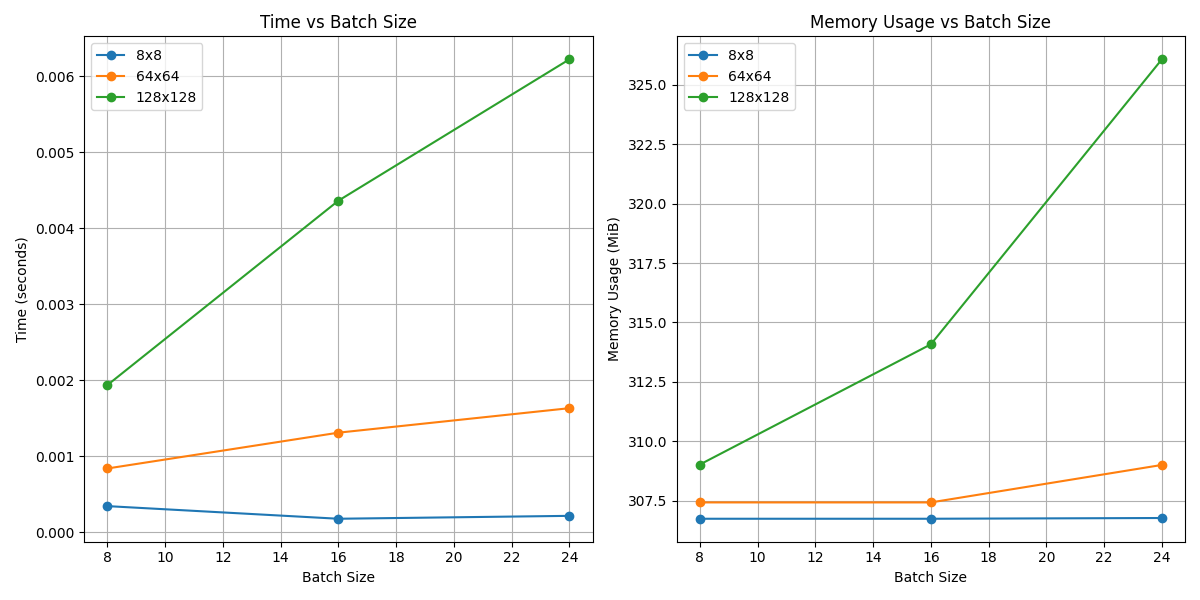
\includegraphics[width=0.8\textwidth]{./figures/denoising_results}
    \caption{Denoising Score Matching Output Graphs}
\end{figure}